\documentclass[12pt]{article}

% a template that a friend gave, it's worked well enough for me
% i have added some packages and stuff that have proved useful

\usepackage{fancyhdr}
\usepackage{tipa}
\usepackage{fontspec}
\usepackage{amsfonts}
\usepackage{enumitem}
\usepackage[margin=1in]{geometry}
\usepackage{graphicx}
\usepackage{float}
\usepackage{amsmath}
\usepackage{braket}
\usepackage{amssymb}
\usepackage{booktabs}
\usepackage{hyperref}
\usepackage{mathtools}
\usepackage{xcolor}
\usepackage{float}
\usepackage{algpseudocodex}
\usepackage{titlesec}
\usepackage{bbm}

\pagestyle{fancy}
\fancyhf{} % sets both header and footer to nothing
\lhead{Kevin Sheng}
\setmainfont{Comic Neue}
\renewcommand{\headrulewidth}{1pt}
\setlength{\headheight}{0.75in}
\setlength{\oddsidemargin}{0in}
\setlength{\evensidemargin}{0in}
\setlength{\voffset}{-.5in}
\setlength{\headsep}{10pt}
\setlength{\textwidth}{6.5in}
\setlength{\headwidth}{6.5in}
\setlength{\textheight}{8in}
\renewcommand{\headrulewidth}{0.5pt}
\renewcommand{\footrulewidth}{0.3pt}
\setlength{\textwidth}{6.5in}
\usepackage{setspace}
\usepackage{multicol}
\usepackage{float}
\setlength{\columnsep}{1cm}
\setlength\parindent{24pt}
\usepackage [english]{babel}
\usepackage [autostyle, english = american]{csquotes}
\MakeOuterQuote{"}

\setlength{\parskip}{6pt}
\setlength{\parindent}{0pt}

\titlespacing\section{0pt}{12pt plus 4pt minus 2pt}{0pt plus 2pt minus 2pt}
\titlespacing\subsection{0pt}{12pt plus 4pt minus 2pt}{0pt plus 2pt minus 2pt}
\titlespacing\subsubsection{0pt}{12pt plus 4pt minus 2pt}{0pt plus 2pt minus 2pt}

\hypersetup{colorlinks=true, urlcolor=blue}

\newcommand{\correction}[1]{\textcolor{red}{#1}}


\rhead{ECE 102}

\newcommand{\rect}{\operatorname{rect}}

\begin{document}

\begin{enumerate}
      \item \begin{enumerate}
                  \item \begin{enumerate}
                              \item 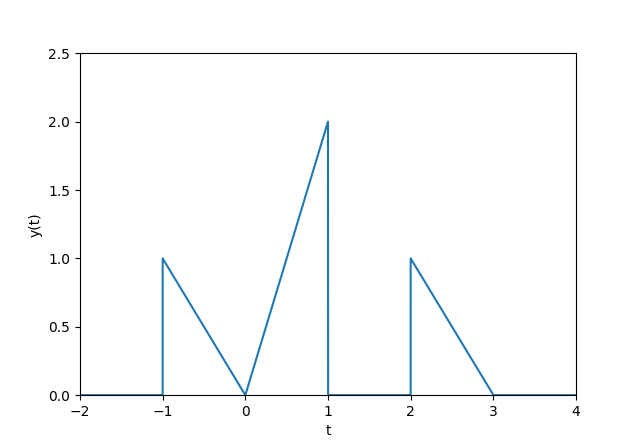
\includegraphics[width=13cm]{img/hw2/i}
                              \item 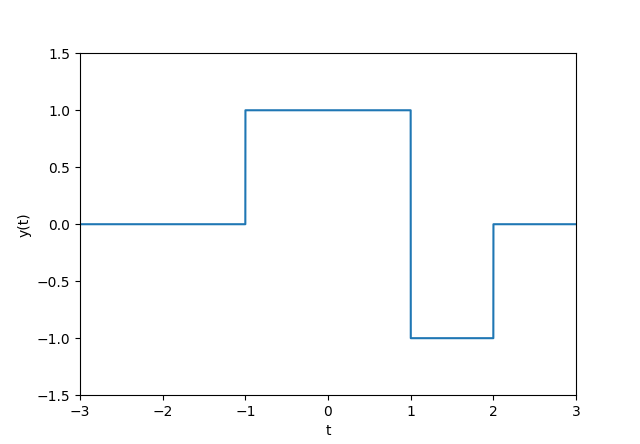
\includegraphics[width=13cm]{img/hw2/ii}
                              \item 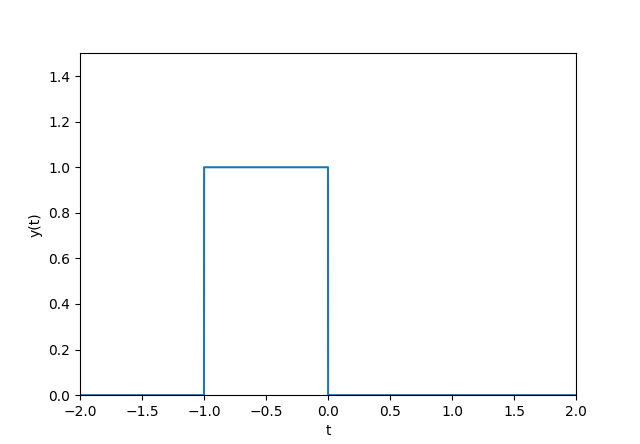
\includegraphics[width=13cm]{img/hw2/iii}
                        \end{enumerate}
                  \item \begin{enumerate}
                              \item \[\begin{aligned}[t]
                                                \int_{-\infty}^{\infty} f(t+1)\delta(t+1)\,dt
                                                 & = \int_{-\infty}^{\infty} f(\tau)\delta(\tau)\,d\tau \\
                                                 & = \boxed{f(0)}
                                          \end{aligned}\]
                              \item The expression is nonzero only when $\tau \ge 1$.
                                    Let's first assume $t \ge 1$:
                                    \[\int_{t}^{\infty} e^{-2\tau}\,d\tau = \left.\left(-\frac{1}{2}e^{-2\tau}\right)\right|^\infty_t = \frac{1}{2}e^{2t}\]
                                    When $t \le 1$, the part from $t$ to $1$ will always be zero.
                                    Thus,
                                    \[f(t)=\begin{cases}
                                                \frac{1}{2}e^{-2}\quad t < 1 \\
                                                \frac{1}{2}e^{-2t}\quad t \ge 1
                                          \end{cases}\]
                              \item \[\begin{aligned}[t]
                                                \int_{0}^{\infty} f(t)(\delta(t-1)+\delta(t+1))\,dt
                                                 & = \int_{0}^{\infty} f(t)\delta(t-1)+f(t)\delta(t+1)\,dt \\
                                                 & = \int_{0}^{\infty} f(t)\delta(t-1)\,dt                 \\
                                                 & = \boxed{f(1)}
                                          \end{aligned}\]
                        \end{enumerate}
                  \item \[\begin{gathered}[t]
                                    \int \delta(bt)\,dt = \int \frac{1}{b}\delta(\tau)\,d\tau=\frac{1}{b}u(t) \\
                                    \int \frac{1}{b}\delta(t)\,dt = \frac{1}{b}u(t)
                              \end{gathered}\]
                        As we can see, the integrals of these two functions are the same.
                        Since they're only nonzero when $t=0$, it is evident that
                        these two functions themselves are also identical. $\quad$
            \end{enumerate}
      \item \begin{enumerate}
                  \item \begin{itemize}
                              \item $2\Delta(t-1)+\Delta(t-2)$
                              \item $\Delta(t+1)+2\Delta(t)+\Delta(t-1)$
                              \item $2\rect(t)+\Delta(t)+2\Delta(t-1)+2\Delta(t+1)$
                        \end{itemize}
                  \item \begin{itemize}
                              \item $u(t)+2u(t-1)-3u(t-3)-4u(t-4)$
                              \item $2u(t-1)-u(t-3)-2u(t-5)+2u(t-7)+u(t-8)$
                        \end{itemize}
            \end{enumerate}
      \item \begin{enumerate}
                  \item \begin{enumerate}
                              \item \textbf{TI:} No.
                                    \begin{align*}
                                          y'(t)       & =|x(t-\alpha)|+x\left(t^2-\alpha\right)            \\
                                          y(t-\alpha) & =|x(t-\alpha)|+x\left|(t-\alpha)^2\right|          \\
                                                      & =|x(t-\alpha)|+x\left(t^2-2t\alpha+\alpha^2\right) \\
                                                      & \ne y'(t)
                                    \end{align*}

                                    \textbf{Causal:} No.
                                    If we need to know, say, $y(2)$, we need to know
                                    $x(2)$ as well as $x\left(2^2\right)=x(4)$.

                                    \textbf{Stable:} Yes.
                                    \begin{gather*}
                                          |x(t)| \le M_x \\
                                          x\left(t^2\right) \le M_x \\
                                          |x(t)|+x(t^2)=y(t) \le 2M_x
                                    \end{gather*}
                              \item \textbf{TI:} Yes.
                                    \begin{align*}
                                          y'(t-\alpha) & =\int_{t-\alpha+T}^{t-\alpha-T} x(\tau)\,d\tau        \\
                                          y'(t)        & = \int_{t+T}^{t-T} x(\tau-\alpha)\,d\tau              \\
                                                       & = \int_{t+T-\alpha}^{t-T-\alpha} x(\lambda)\,d\lambda \\
                                                       & = y'(t)
                                    \end{align*}

                                    \textbf{Causal:} No. $y(t)$ depends on some future values like $x(t+T)$ for the integral.

                                    \textbf{Stable:} Yes.
                                    \begin{gather*}
                                          |x(t)| \le M_x \\
                                          \int_{t+T}^{t-T} |x(\tau)|\,d\tau \le 2TM_x \\
                                          \int_{t+T}^{t-T} x(\tau)\,d\tau=y(t) \le 2TM_x
                                    \end{gather*}
                              \item \textbf{TI:} No.
                                    \begin{align*}
                                          y(t-\alpha) & =(t-\alpha+1)\int_{-\infty}^{t-\alpha} x(\lambda)\,d\lambda \\
                                          y'(t)       & =(t+1)\int_{-\infty}^{t} x(\lambda-\alpha)\,d\lambda        \\
                                                      & = (t+1) \int_{-\infty}^{t-\alpha} x(\tau)\,d\tau            \\
                                                      & \ne y(t-\alpha)
                                    \end{align*}

                                    \textbf{Causal:} Yes.
                                    $y(t)$ only needs to know values from $-\infty$ to $t$.

                                    \textbf{Stable:} No.
                                    $x(t)=1$ is a counterexample.
                                    \[y(0)=\int_{-\infty}^{0}1\,d\tau=\infty\]
                              \item \textbf{TI:} Yes.
                                    \begin{gather*}
                                          y'(t)=1+e^{x(t-\alpha)} \\
                                          y'(t-\alpha)=1+e^{x(t-\alpha)}= y'(t)
                                    \end{gather*}

                                    \textbf{Causal:} Yes.
                                    $y(t)$ only depends on the current value of $x(t)$.

                                    \textbf{Stable:} Yes.
                                    \begin{gather*}
                                          |x(t)| \le M_x \\
                                          e^{x(t)} \le e^{M_x} \\
                                          1+e^{x(t)}=y(t) \le 1+e^{M_x}
                                    \end{gather*}
                              \item \textbf{TI:} Yes.
                              \begin{gather*}
                                    y'(t) = \frac{1}{1+x(t-\alpha)^2} \\
                                    y(t-\alpha)=\frac{1}{1+x(t-\alpha)^2}=y'(t)
                              \end{gather*}

                                    \textbf{Causal:} Yes.
                                    $y(t)$ only depends on the current value of $x(t)$.

                                    \textbf{Stable:} Yes.
                                    \begin{gather*}
                                          x(t)^2 \ge 0 \\
                                          \frac{1}{1+x(t)^2} \le 1
                                    \end{gather*}
                        \end{enumerate}
                  \item \[\begin{aligned}[t]
                                    z(t)
                                     & =\int_{-\infty}^{t} x\left(\frac{\tau}{2}\right)\,d\tau                                              \\
                                     & = \int_{-\infty}^{t/2} 2x(\lambda)\,d\lambda            & \text{Substitute }\lambda = \frac{\tau}{2}
                              \end{aligned}\]
                        For the desired signal, our final system $y(t)$ must be
                        \[\boxed{y(t)=\frac{1}{2}z(2t-2)}\]
                  \item \begin{enumerate}
                              \item Let the system after $\mathcal{S}_1$ and
                                    $\mathcal{S}_2$ be $w(t)$ and $y(t)$ respectively.
                                    A shift of $x(t)$ by $\alpha$ will produce $w(t-\alpha)$.
                                    Since $\mathcal{S}_2$ is also TI, inputting $w(t-\alpha)$ into it
                                    will produce a corresponding $y(t-\alpha)$.

                                    Thus, the series cascade of $\mathcal{S}_1$ and $\mathcal{S}_2$ is TI. $\square$
                              \item Let the system after $\mathcal{S}_1$ and
                                    $\mathcal{S}_2$ be $w(t)$ and $z(t)$ respectively.
                                    In shifting $x(t)$ by $\alpha$, we make the outputs $w(t-\alpha)$ and $z(t-\alpha)$.
                                    \[y(t) = w(t) + z(t) \therefore y(t - \alpha) = w(t -\alpha) + z(t-\alpha)\quad\square\]
                        \end{enumerate}
            \end{enumerate}
      \item \begin{enumerate}
                  \item Let's first compute $|x(t)|^2$.
                        \begin{align*}
                              Ae^{j\omega t}+Be^{-j\omega t}
                               & = e^{j\phi}\left(r_1e^{j\omega t}+r_2e^{-j\omega t}\right)               \\
                               & = e^{j\phi}\left((r_1+r_2)\cos(\omega t)+j(r_1-r_2)\sin(\omega t)\right)
                        \end{align*}
                        The magnitude of $e^{j\phi}$ is $1$, so it doesn't contribute anything.
                        Considering only the expression in parenthesis,
                        the square of its magnitude is
                        \[((r_1+r_2)\cos(\omega t))^2+((r_1-r_2)\sin(\omega t))^2
                              = r_1^2+r_2^2 + 2r_1r_2(\cos^2(\omega t)-\sin^2(\omega t))\]

                        Taking the integral, we get that it's
                        \begin{align*}
                              &\hphantom{={}} \int_{-T}^T r_1^2+r_2^2+2r_1r_2(\cos^2(\omega t)-\sin^2(\omega t)) \\
                              &= 2T(r_1^2+r_2^2)+\int_{-T}^{T} \cos^2(\omega t)-\sin^2(\omega t)\,dt \\
                              &= 2T(r_1^2+r_2^2)+\int_{-T}^{T} \cos(2\omega t)\,dt \\
                              &= 2T(r_1^2+r_2^2)
                        \end{align*}
                        As $T \to \infty$, this expression also diverges,
                        but $\frac{1}{2T}$ times the expression gives a constant value.

                        Thus, this is a power signal with average power $\boxed{r_1^2+r_2^2}$.
                  \item \[\begin{aligned}[t]
                                    \exp(-t(1+j\omega_1+j\omega_2))
                                     & = e^{-t}\exp(-tj(\omega_1+\omega_2))                           \\
                                     & = e^{-t}(\cos(t\omega_1+t\omega_2)-j\sin(t\omega_1+t\omega_2))
                              \end{aligned}\]
                        This signal has squared magnitude $e^{-2t}$ when $t \ge -1$ $0$ otherwise.
                        \[\int_{-1}^{\infty} e^{-2t}\,dt = \left.\left(-\frac{1}{2}e^{-2t}\right)\right|^{\infty}_{-1}=\frac{e^2}{2}\]
                        This is an energy signal with energy $\boxed{\frac{e^2}{2}}$.
            \end{enumerate}
      \item After this PDF will be the Jupyter Notebook I ran.
\end{enumerate}
\end{document}
